%% -*- coding: utf-8-unix -*-

\chapter{NetTesterの使いかた}
\label{chap:nettester-usage}

 \section{NetTesterのデプロイ}
 \label{sec:nettester-deployment}

  \subsection{物理OpenFlowスイッチ}
  \label{sec:nettester-deploy-psw}

  % 物理OFSのデプロイ
  % - pica8 (OVS) の設定について
  %   - Portの設定(VLAN) : [L1PJTECH] 参照
  %   - \code{fail\_mode} の設定
  %     \url{https://docs.google.com/document/d/1yBn8S3DOhkuaVuVtUmwOeyvQxWm1v6_PfWTj3iDcx0U/}
  %   - inactivity probe の設定:
  %     調査: テスト環境でOFS(Pica8)-OFC(NetTester/Trema)の接続が切れる – NetTester
  %     \url{https://3.basecamp.com/3088280/buckets/867009/todos/218484578}
  %     \url{https://docs.google.com/document/d/1_-pLOXSOLutRb1_-tlcb_FwLCHq3Y7zQxp79_qXjDiM/}
  %     (そんなに重要じゃないけど一応)

\ref{sec:nettester-model}節に示したとおり、NetTester は1台の物理OpenFlow
スイッチを利用して、テスト対象ネットワークへの接続をおこなう(物理
OpenFlowスイッチを使用してテストトラフィックを''distribute''する)。本節
では物理OpenFlowスイッチの選択と設定について解説する。

% NetTesterが使用する物理OpenFlowスイッチには\tabref{tab:ofs-requirement}
% の要件が求められる~\cite{l1pjpoc}。

\begin{table}[h]
 \centering
 \caption{OpenFlowスイッチ要件(OpenFlow/1.0)}
 \label{tab:ofs-requirement}
 \begin{tabular}{l|l}
  \hline
  分類 & 項目 \\
  \hline
  \hline
  Match  & In-Port \\ \cline{2-2}
         & VLAN ID \\ \cline{2-2}
         & Source/Destination MAC Address \\ \hline
  Action & Out-Port \\ \cline{2-2}
         & Push/Pop VLAN ID \\ \hline
  Priority & Priority \\
  \hline
 \end{tabular}
\end{table}

本プロジェクトでは昨年度実施した \lopj の環境を継続しており、
\tabref{tab:psw-list}に示すOpenFlowスイッチを使用している~\cite{l1pjpoc}。
(2台のOpenFlowスイッチを使用して Tester set を2セット構築している。)
% TODO: Tester set の説明

\begin{table}[h]
 \centering
 \caption{物理OpenFlowスイッチ}
 \label{tab:psw-list}
  \begin{tabular}{l|l|l}
   \hline
   Host name & Hardware & OS/Version \\
   \hline
   \hline
   OFS1 & Quanta T1048-LB9 & PicOS 2.5.2 / Revision 19975 \\
   OFS2 & Pica8 P-3290 & PicOS 2.2.1S3 / Revision 14775 \\
   \hline
 \end{tabular}
\end{table}
% TODO: 昨年度ドキュメントそのまま。現物確認すること
% TODO: OVS version を追記すること。

PicOSはOVS Mode (Open vSwitch)で使用する。PicOS OVSでは以下の設定をおこ
なう。下記設定事項についてはPicOSマニュアルおよびOpen vSwitchドキュメン
ト\footnote{ovs-vswitchd.conf.db.5.txt
\url{http://openvswitch.org/support/dist-docs/ovs-vswitchd.conf.db.5.txt}}
も参照すること。
\begin{itemize}
 \item パッチとして使用するすべてのポートの設定~\cite{l1pjtech}
       \begin{itemize}
        \item VLANの操作をおこなうため、VLAN Mode を trunk として設定
              (\verb|vlan_mode=trunk|)する:
        \item テスト対象ネットワークで発生するブロードキャスト転送の抑制・
              STPへの干渉をさけるため、フラッディングの無効化
              (\verb|no-flood|)およびSTPの無効化(\verb|no-stp|)を設定す
              る。
       \end{itemize}
 \item 物理OpenFlowスイッチ(OVS Bridge)全体の設定
       \begin{itemize}
        \item BridgeでSTPを処理しない(\verb|stp_enable=false|)。
        \item コントローラ(OFC)との接続が切断された際にテスト対象ネット
              ワークから届くトラフィックを処理しない
              (\verb|fail_mode=secure|)\footnote{\code{fail\_mode}には
              secureとstandaloneの2種類がある。Standaloneを指定した場合、
              OFS(OVS Bridge)はOFCとの接続がきれた際に独立したL2スイッチ
              (Learning Switch)として動作する。テスト対象ネットワークと
              の物理結線がある状態でL2スイッチとして動作してしまうと、テ
              スト対象ネットワークをまきこんでL2ループが発生してしまうた
              め注意が必要である。}\footnote{PicOSでは、PicOSバージョン
              が異なると(PicOS上のOVSのバージョンが同一でも)OVSの
              \code{fail\_mode}デフォルト設定が異なっているため注意が必
              要である。利用する場合は明示的に\code{fail\_mode=secure}を
              設定すること。}。
        \item (Optional) 物理OpenFlowスイッチとOFC(NetTester OFC)との接
              続がタイミングにより切断されるなどの現象がある場合には、
              Inactivity probe の値を調整する。
       \end{itemize}
\end{itemize}

  
  \subsection{NetTester Server の構成選択}
  \label{sec:nettester-server-deploy-pattern}

  % NetTesterモデルの制約とサーバ構成の選択肢
  % - 必要なNIC
  % - ベアメタル
  % - KVM による仮想化, その場合のNIC設定

NetTesterサーバは物理OpenFlowと物理リンクで直結される必要がある。サーバ
の構成方法として、ベアメタル構築する場合と仮想マシンで構築する場合の注意
事項について解説する。

\paragraph{ベアメタル構成}
NetTesterサーバをベアメタルで構成する場合は
\figref{fig:nettester-deploy-baremetal}のようになる。
\ref{sec:nettester-model}節に示したとおり、NetTesterサーバと物理スイッチ
(PSW)間は物理リンクで直結される必要がある。また、OpenFlowチャネルや
NetTester-PSW間の制御・管理通信のために、NetTesterサーバとPSWは管理ネッ
トワークを介して通信をおこなう。
\begin{figure}[h]
 \centering
 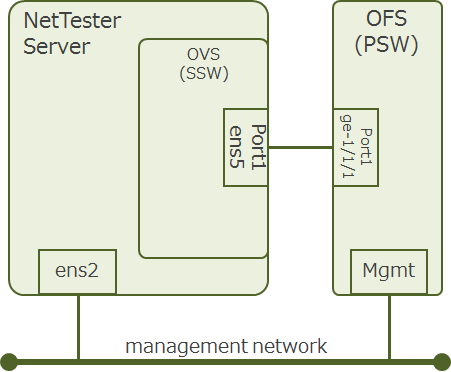
\includegraphics[scale=0.6]{img/nettester-deploy-baremetal.png}
 \caption{ベアメタル構成}
 \label{fig:nettester-deploy-baremetal}
\end{figure}

\paragraph{仮想マシン構成}
NetTesterサーバを仮想マシンとして構成する場合は
\figref{fig:nettester-deploy-vm}のようになる。管理ネットワークについては
ベアメタル構成の場合と同様にL2/L3でPSWとのコネクティビティがとれればよい。
NetTester(SSW)-PSW間の接続については、ホストOS側で物理ポート(リンク)を
NetTesterサーバ(VM)へ直結させる必要がある。SSW-PSW間はOFC(NetTester)によっ
て制御するため、ハイパーバイザ側ではL2以上の制御はおこなわない。パススルー
あるいはプロミスキャスモードで接続する。

\begin{figure}[h]
 \centering
 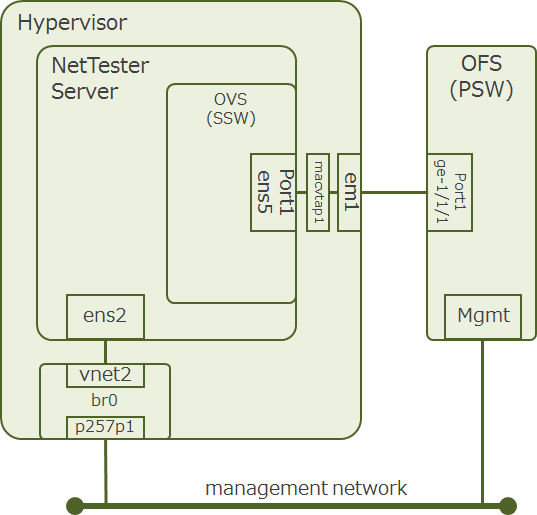
\includegraphics[scale=0.6]{img/nettester-deploy-vm.png}
 \caption{仮想マシン構成}
 \label{fig:nettester-deploy-vm}
\end{figure}

本プロジェクトは仮想マシン構成を採用した。PoCでは
\tabref{tab:server-spec}に示すサーバを使用している。SSW-PSW間接続では、
ハイパーバイザ(KVM Host)が持つ物理NICを直接仮想マシンに接続
(\code{macvtap/passthrough})させる(\lstref{lst:kvmconf-psw-port})。管理
ネットワークについては bridge 接続でよい(他のVMやハイパーバイザとL2で接
続する, \lstref{lst:kvmconf-mgmt-port})。

\begin{table}[h]
 \centering
 \caption{サーバ情報}
 \label{tab:server-spec}
 \begin{tabularx}{\linewidth}{l|X|X}
  \hline
  Host & OS & Virtualization \\
  \hline
  \hline
  \shortstack[l]{Hypervisor\\(KVM Host)}
    & \shortstack[l]{Ubuntu 14.04.5 LTS\\(GNU/Linux 3.16.0-30-generic x86\_64)}
    & \shortstack[l]{qemu-kvm/2.0.0+dfsg-2ubuntu1.25,\\libvirt/1.2.2-0ubuntu13.1.17} \\
  \hline
  \shortstack[l]{NetTester Server\\(VM)}
    & \shortstack[l]{Ubuntu 16.04.1 LTS\\(GNU/Linux 4.4.0-31-generic x86\_64)}
    & \\
  \hline
 \end{tabularx}
\end{table}

\begin{lstlisting}[language=xml,caption=PSW接続用ポート設定,label=lst:kvmconf-psw-port]
<interface type='direct'>
  <mac address='52:54:00:12:56:0e'/>
  <source dev='em1' mode='passthrough'/>
  <target dev='macvtap1'/>
  <model type='virtio'/>
  <alias name='net1'/>
  <address type='pci' domain='0x0000' bus='0x00' slot='0x05' function='0x0'/>
</interface>
\end{lstlisting}
\begin{lstlisting}[language=xml,caption=管理ポート設定,label=lst:kvmconf-mgmt-port]
<interface type='bridge'>
  <mac address='52:54:00:64:ee:38'/>
  <source bridge='br0'/>
  <target dev='vnet2'/>
  <model type='virtio'/>
  <alias name='net0'/>
  <address type='pci' domain='0x0000' bus='0x00' slot='0x02' function='0x0'/>
</interface>
\end{lstlisting}


  \subsection{NetTester Server のソフトウェアスタック}

  % 必要なソフトウェア(package)とインストール
  % - 基本的なパッケージ
  %   - open vswitch
  %   - ruby, rubyenv
  %   - Git
  %   - Build-Essentials
  %   - テストシナリオでつかうもの (nc, dnsmasqなど)
  % - OSの設定
  %   - sudoers secure\_path

  \subsection{テストシナリオ (net-tester/examples)}

  \subsection{NetTester}

\section{基本的な使い方}

NetTester 単独での利用
\begin{itemize}
 \item NetTesterでad-hocなテスト作業を拡張する - Qiita \url{http://qiita.com/corestate55/items/d6a8cdc03de09a46877c}
       これの基礎編のところをいれておけばよいとおもわれる
 \item 環境変数の設定
       \begin{itemize}
        \item ``DEVICE``
              \begin{itemize}
               \item 調査:セグメントローカルの試験がとおらない – NetTester \url{https://3.basecamp.com/3088280/buckets/867009/todos/259184454}
               \item ネットワークデバイスと dpid を rake に渡せるようにする – NetTester \url{https://3.basecamp.com/3088280/buckets/867009/todos/214833956}
              \end{itemize}
        \item expectacle 関連
       \end{itemize}
\end{itemize}

%%% Local Variables:
%%% mode: yatex
%%% TeX-master: "main.tex"
%%% End:
